% template cloned from https://gitlab.kit.edu/kit/kastel/sdq/dokumentvorlagen/praesentationen/beamer
% commit: 7960880f39b47ec10eabeed2baf9468fb38312a5 (Mar 4, 2025)

\documentclass[en, navbaroff, handout]{sdqbeamer}
% class options:
% - language: de (default), en
% - navbar can be toggled on (default) / off
% - footer font size: bigfoot (default), smallfoot (KIT layout)
% - font for slide titles: franklin (default) / helvet
% - show lines for alignining content on slides: kitgrid
% - remove animation roll-out: handout (general "beamer" option, not specific for this class)

\grouplogo{} % needs to be empty to be turned off
\groupname{} % empty allows author and title to take more space
%\groupnamewidth{89mm} % default

\title[Subgroup Discovery with Small and Alternative Feature Sets]{Subgroup Discovery with Small and Alternative Feature Sets} % [footer]{title slide}
\subtitle{SIGMOD 2025 | Berlin} 
\author[Jakob Bach]{Jakob Bach} % [footer]{title slide}

\date[2025-06-24]{June 24, 2025} % [footer]{title slide}

%\usepackage{amsmath} % mathematical symbols and equations; apparently pre-loaded
%\usepackage{amssymb} % mathematical symbols; apparently pre-loaded
\usepackage[style=numeric, backend=bibtex]{biblatex}  % original template uses "biber" as backend
\usepackage{booktabs} % nicely formatted tables (with top, mid, and bottom rule)
%\usepackage{graphicx} % plots; apparently pre-loaded
\usepackage{multirow} % cells spanning multiple rows in tables
\usepackage{subcaption} % subfigures
\usepackage{tikz} % used for non-float figure positioning
%\usepackage{hyperref} % links and URLs; apparently pre-loaded

\addbibresource{references.bib}

\hypersetup{colorlinks=true, citecolor=kit-blue, urlcolor=kit-blue}
 
\setlength{\leftmargini}{0.6cm} % change default indentation (so first-level items are left-aligned to boxes and slide titles)

\setbeamerfont{itemize/enumerate subbody}{size=\normalsize} % make 2nd-level items' text as large as 1st-level ones (default is \small, as defined in "beamerfontthemedefault.sty")
\setbeamerfont{itemize/enumerate subsubbody}{size=\normalsize} % make 3rd-level items' text as large as 1st-level ones (default is \footnotesize, as defined in "beamerfontthemedefault.sty")

% make bullet points slightly smaller and roughly center them relative to upper-case letters (instead of bottom alignment):
\setbeamertemplate{itemize item}{\raisebox{2.17pt}{\color{kit-green}\footnotesize$\blacksquare$}}
\setbeamertemplate{itemize subitem}{\raisebox{2.17pt}{\color{kit-green}\scriptsize$\blacksquare$}}
\setbeamertemplate{itemize subsubitem}{\raisebox{2.17pt}{\color{kit-green}\scriptsize$\blacksquare$}}

\setbeamercovered{invisible} % can set "transparent" to show later content of animated slide in gray

\begin{document}

\begin{frame}[title white horizontal, kitlogo=rgb]
	% layout options: "white horizontal", "green horizontal", "white vertical", "blue vertical"
	% KIT logo options: rgb, white, black
	\titlepage
\end{frame}

\section{Talk}

\begin{frame}[t]{Subgroup Discovery}
	\begin{itemize}
		\item \textbf{Subgroup discovery:} ``Identifying descriptions of subsets of a dataset that show an interesting behavior''~\cite{atzmueller2015subgroup}
		%JB: unlike typical ML prediction models, need not cover full dataset with one subgroup (there may be multiple ones)
		\begin{itemize}
			\item Language for descriptions typically simple
			%JB: e.g., restrict ranges of numerical features or select particular values of categorical features
			\item `Interesting' according to some objective function
			%JB: notion of subgroup quality
		\end{itemize}
		\pause
		\vspace{\baselineskip}
		\item \textbf{Our scope:} Binary classification with real-valued features
		\begin{itemize}
			\item Tabular dataset $X \in \mathbb{R}^{m \times n}$ (data objects $\times$ features)
			%JB: there also are variants of subgroup discovery that are more like frequent itemset mining, with binary feature values and only value 1 used in subgroup descriptions
			\item Prediction target $y \in \{0, 1\}^m$ (`interesting'/`positive' = 1)
			%JB: in regression, interestingness could refer to low or high values of target
			\pause
			\item Subgroup description: Hyperrectangle
			\item Subgroup quality: Weighted Relative Accuracy
			\begin{itemize}
				\item $\text{WRAcc} = \frac{m_b}{m} \cdot \left( \frac{m_b^+}{m_b} - \frac{m^+}{m} \right)$~\cite{lavravc1999rule}
				%JB: first factor is subgroup size, second is relative accuracy (precision in subgroup vs overall)
				\item \emph{+} $\leftrightarrow$ positive data object, \emph{b} $\leftrightarrow$ in subgroup (box)
			\end{itemize}
		\end{itemize}
		\pause
		\vspace{\baselineskip}
		\item \textbf{Our goal}: Introduce and analyze two constraint types to foster interpretability of subgroup descriptions
		%JB: constraints on selected features
		%JB: despite subgroup descriptions already being simple
		\begin{itemize}
			\item Limit number of features used in subgroup description
			%JB: "small"
			%JB: imagine dataset with 100 dimensions and all are bounded
			%JB: kind of extension to traditional feature selection in ML (one binary decision for each feature; now values play a role)
			\item Find alternative subgroup descriptions
			%JB: "alternative"
			%JB: alternative description for same subgroup, not an alternative subgroup
		\end{itemize}
	\end{itemize}
	\pause[0] % \visible or \onslide did not work, so we reset pause counter to show figure immediately
	\begin{tikzpicture}[remember picture,overlay]
		\node[xshift=-260pt,yshift=-310pt] at (current page.north east) {
			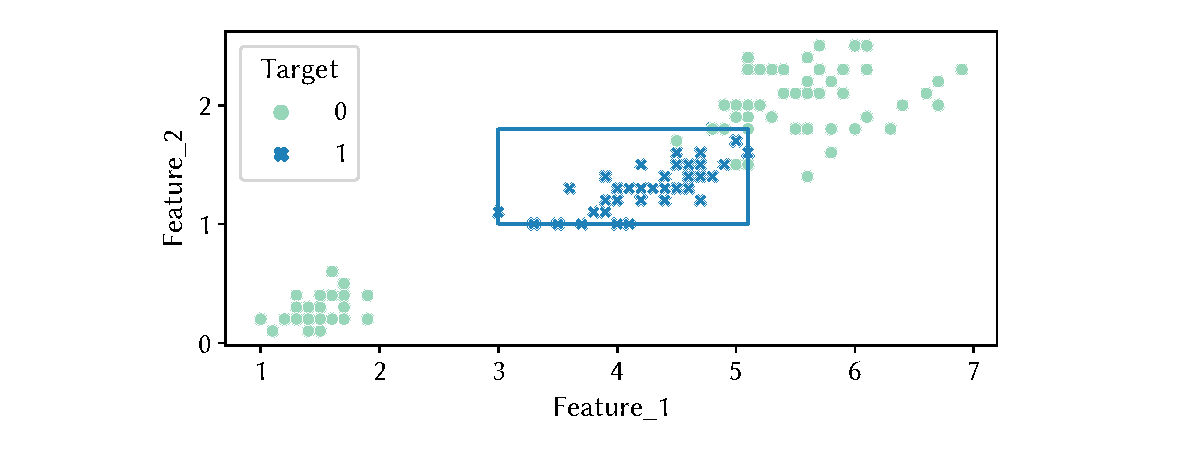
\includegraphics[width=0.45\textwidth, trim=70 15 90 15, clip]{plots/csd-exemplary-subgroup.pdf}
		};
	\end{tikzpicture}
\end{frame}

\begin{frame}[t]{Contributions and Related Work}
	\begin{itemize}
		\item \textbf{Contributions:}
		%JB: formalization, proofs, and experiments
		\begin{itemize}
			\item Formalize subgroup discovery as an SMT (Satisfiability Modulo Theories) optimization problem
			%JB: can be tackled with a solver instead of needing to develop a problem-specific algorithm (which may need further adaptation for particular constraint types)
			\item Formalize two constraint types:
			%JB: the two points mentioned on previous slide
			%JB: all following contributions are for both constraint types each
			\begin{itemize}
				\item Feature-cardinality constraints
				\item Alternative subgroup descriptions
			\end{itemize}
			%JB: besides SMT formalization, also show how to integrate constraints into existing, heuristics subgroup-discovery methods
			\item Analyze computational complexity and show $\mathcal{NP}$-hardness
			%JB: unfortunately, no time for these proofs in this 15-min presentation; one proof is in Appendix of this presentation
			\item Comprehensive experiments
			% will be presented later
		\end{itemize}
		\pause
		\vspace{\baselineskip}
		\item \textbf{Related work:}
		\begin{itemize}
			\item Existing subgroup-discovery methods~\cite{atzmueller2015subgroup, helal2016subgroup, herrera2011overview, ventura2018subgroup} typically algorithmic (exhaustive or heuristic)
			%JB: i.e., exhaustive routines do not use an off-the-shelf solver
			%JB: further, term "subgroup" is a bit overloaded; also used in algorithmic fairness (predefined groups like race, gender), medicine, and re-inventions with slightly different problem definitions in different communities (like management of data)
			\item Few white-box formulations of (other) variants of subgroup discovery~\cite{bonates2008maximum, eckstein2002maximum, guns2011itemset, koccak2020exploiting, louveaux2014combinatorial}
			%JB: typically evaluation limited, e.g., not comparing to existing SD methods
			%JB: also, different problem definitions (e.g., further constraints) and neither feature cardinality nor alternatives
			\item Concept of feature cardinality well-established~\cite{herrera2011overview, meeng2021real}, but empirical studies varying it~\cite{friedman1999bump, lemmerich2010fast, meeng2021real, proencca2022robust} are limited
			%JB: e.g., just one SD method
			%JB: some studies also use just one fixed cardinality
			%JB: don't want to say that studies narrow in general; just have a different focus
			\item Concept of alternative subgroups well-established~\cite{atzmueller2015subgroup, belfodil2019fssd, bosc2018anytime, leeuwen2012diverse, lucas2018ssdp+}, but alternative descriptions~\cite{boley2009non, galbrun2017redescription, leeuwen2012diverse, lopez2023discovering} less
			%JB: former (also called "diverse") wants to capture different data objects / regions, not use different features
			%JB: the referenced related work for alternative descriptions pursues different problem definitions than we do
			%JB: alternatives are also a theme in other fields of ML, e.g., clustering, itemset mining, feature selection, and XAI
		\end{itemize}
	\end{itemize}
\end{frame}

\begin{frame}[t]{Formalization -- Basic Problem}
	\vspace{-\baselineskip} % by default, equations are placed lower on slide
	%JB: basic problem is "unconstrained" in sense of no additional constraints apart from ones inherent in problem
	%JB: forms basis for adding feature-cardinality constraints
	\begin{align*}
		\onslide<5->{
			\max &\quad & Q_{\text{WRAcc}} &= \frac{m_b^+}{m} - \frac{m_b \cdot m^+}{m^2} \tag*{(Objective: subgroup quality)} \\
			%JB: we have seen this formula two slides ago (only a bit rearranged now)
			%JB: linear since "m" and "m+" constant
		}
		\onslide<4->{
			\text{s.t.:} &\quad & m_b &:= \sum_{i=1}^{m} b_i \quad\text{and}\quad m_b^+ := \sum_{\substack{i \in \{1, \dots, m\} \\ y_i = 1 }} b_i \tag*{(Num of data objects in subgroup)} \\
			%JB: count b_i
		}
		\onslide<3->{
			&\quad \forall i \in \{1, \dots, m\} & b_i &\leftrightarrow \bigwedge_{j \in \{1, \dots, n\}} \left( \left( X_{ij} \geq \mathit{lb}_j \right) \land \left( X_{ij} \leq \mathit{ub}_j \right) \right) \tag*{(i-th data object in subgroup?)} \\
		}
		\onslide<2->{
			&\quad \forall j \in \{1, \dots, n\} & \mathit{lb}_j &\leq \mathit{ub}_j \tag*{(Constraint: relationship between bounds)} \\
			%JB: technically, you could even leave constraint out in most situations, as solutions with UB < LB would contain zero data objects in box and therefore have WRAcc = 0, while even a box containing only one positive data object (and nothing else) has a WRAcc > 0; however, if feature values of all positive objects also exist with negative labels (no separation possible) and also there is no option to form an empty box (i.e., all combinations of feature values exist in caetgorical scenario), then best WRAcc may become < 0 (and we want this box instead of an invalid one with WRAcc = 0)
		}
		\onslide<3->{
			&\quad & b &\in \{0, 1\}^m \tag*{(Auxiliary variables: subgroup membership)}  \\
			%JB: not strictly necessary (expressions above could be inlined), but we used variables in implementation (though not for m_b and m_b^+, which therefore have := in definition)
			%JB: b_i are also used when defining problem for alternative subgroup descriptions
		}
		\onslide<1->{
			&\quad & \mathit{lb}, \mathit{ub} &\in \{\mathbb{R} \cup \{-\infty, +\infty\}\}^n \tag*{(Variables: lower/upper bounds of subgroup)}
		}
	\end{align*}
\end{frame}

\begin{frame}[t]{Formalization -- Feature-Cardinality Constraints}
	\begin{itemize}
		\item \textbf{Concept:} Limit number of features used (= selected) in subgroup description to $k \in \mathbb{N}$
		%JB: "k" is a user parameter
		%JB: theoretical result: problem is NP-hard under mild assumption on objective function
		\item \textbf{Formally:} Limit number of features whose bounds exclude at least one data object from subgroup
		%JB: i.e., technically, a feature appearing in subgroup description may still not be selected (cannot happen in our implementation because we post-process bounds of subgroups accordingly)
		%JB: e.g., imagine lower bound at -5 while feature has range [0, 10] -> bound not active
		\pause
		\begin{equation*}
			\begin{aligned}
				\onslide<3->{
					\forall j \in \{1, \dots, n\}: && s^{\text{lb}}_j &\leftrightarrow \left( \mathit{lb}_j > \min_{i \in \{1, \dots, m\}} X_{ij} \right) \\
					\forall j \in \{1, \dots, n\}: &&s^{\text{ub}}_j &\leftrightarrow \left( \mathit{ub}_j < \max_{i \in \{1, \dots, m\}} X_{ij} \right) \\
					%JB: min and max feature values are constants here
				}
				\onslide<4->{
					\forall j \in \{1, \dots, n\}: && s_j &\leftrightarrow \left( s^{\text{lb}}_j \lor s^{\text{ub}}_j \right) \\
				}
				\onslide<5->{
					&& \sum_{j=1}^n s_j &\leq k \\
				}
				\onslide<2->{
					&& s, s^{\text{lb}}, s^{\text{ub}} &\in \{0, 1\}^n \\
					%JB: like b_i, these variables are not strictly necessary (could be inlined) but our implementation uses them
				}
			\end{aligned}
		\end{equation*}
	\end{itemize}
\end{frame}

\begin{frame}[t]{Experimental Design}
	\begin{itemize}
		\item \textbf{27 binary-classification datasets} (with 106--9822 data objects and 20--168 features) from \emph{PMLB}~\cite{olson2017pmlb, romano2021pmlb}
		\pause
		\vspace{\baselineskip}
		\item \textbf{Eight subgroup-discovery methods:}
		\begin{itemize}
			\item Solver-based (novel): \emph{SMT} (using \emph{Z3}~\cite{bjorner2015nuz, deMoura2008z3} as optimizer)
			\item Exhaustive search (related work): \emph{BSD}~\cite{lemmerich2010fast}, \emph{SD-Map}~\cite{atzmueller2006sd}
			%JB: not actually exhaustive in our scenario since they require discretizing numeric features
			\item Heuristics (related work): \emph{Beam}, \emph{BI}~\cite{mampaey2012efficient}, \emph{PRIM}~\cite{friedman1999bump}
			%JB: iteratively and greedily restrict the subgroup's bounds, with one feature per iteration (PRIM: prune fixed fraction of data objects; Beam/BI: test all possible cuts)
			\item Baselines (novel): \emph{MORS} (Minimal Optimal Recall Subgroup), \emph{Random}
			%JB: MORS -- minimal bounds such that all positive data objects are in subgroup (exclude as many negative data objects as possible); intermediate problem between SD and perfect SD
			%JB: Random -- repeated random sampling of bounds
		\end{itemize}
		\pause
		\vspace{\baselineskip}
		\item \textbf{Experimental scenarios:}
		%JB: parameters varied systematically; all other hyperparameters fixed, i.e., no tuning
		\begin{itemize}
			\item Solver timeouts: \{1~s, 2~s, 4~s, $\dots$, 2048~s\}
			\item Feature-cardinality constraints: $k \in \{1, 2, 3, 4, 5\}$
			\item Alternative subgroup descriptions: $k=3$ features, $a=5$ alternatives, and dissimilarity threshold $\tau_{\text{abs}} \in \{1, 2, 3\}$
			%JB: do not have time to describe details; in a nutshell: find $a$ other subgroup descriptions that should capture a similar set of data objects as a given description but use different features
		\end{itemize}
		\pause
		\vspace{\baselineskip}
		\item \textbf{Evaluation metrics:}
		\begin{itemize}
			\item Subgroup quality (nWRAcc~\cite{lavravc1999rule, mathonat2021anytime})
			%JB: normalized version of WRAcc we discussed before (takes dataset imbalance into account, always has range [-1, 1])
			\item Runtime
			\item For alternatives: Similarity~\cite{choi2010survey} (Normalized Hamming and Jaccard)
		\end{itemize}
	\end{itemize}
\end{frame}

\begin{frame}[t]{Results -- Feature-Cardinality Constraints}
	\begin{figure}
		\centering
		\begin{subfigure}[t]{0.32\textwidth}
			\centering
			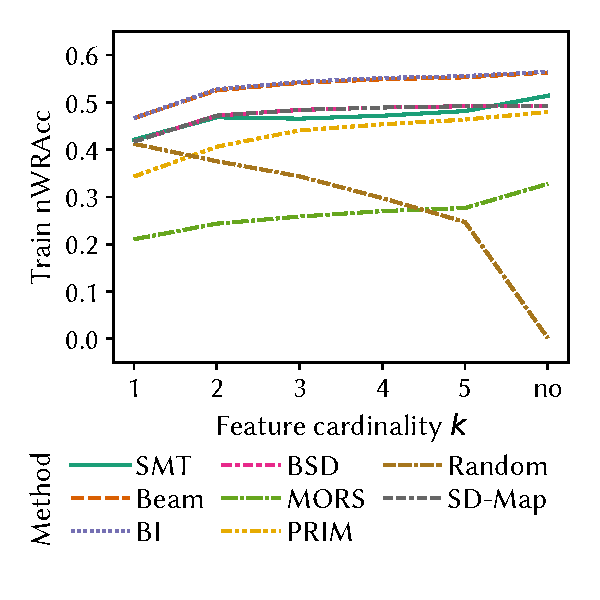
\includegraphics[width=\textwidth, trim=10 25 10 10, clip]{plots/csd-cardinality-train-nwracc-all-datasets.pdf}
			\caption{All 27 datasets, training set.}
			\label{fig:csd:cardinality-train-nwracc-all-datasets}
			%JB: on average, heuristics "Beam" (orange) and "BI" (purple) beat solver-based search "SMT" (dark green) due to timeouts (here, largest timeout setting of 2048~s)
			%JB: "exhaustive" competitors "BSD" (pink) and "SD-Map" (gray) comparable to SMT (dark green), suffer from discretization (we apply their built-in equal-with binning and optimize over different number of bins, but still way smaller search space than being allowed to choose bounds arbitrarily)
			%JB: other baselines and heuristics ("PRIM", "Random", "MORS") worse
			%JB: increase of subgroup quality over "k" is small, i.e., small subgroup descriptions (with just 1 or 2 out of >= 20 features) already yield high quality (encouraging for interpretability)
		\end{subfigure}
		\pause
		\hfill
		\begin{subfigure}[t]{0.32\textwidth}
			\centering
			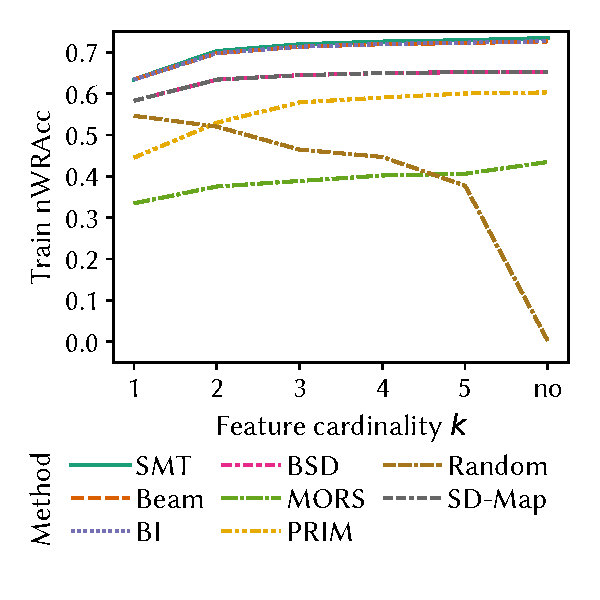
\includegraphics[width=\textwidth, trim=10 25 10 10, clip]{plots/csd-cardinality-train-nwracc-no-timeout-datasets.pdf}
			\caption{13 datasets without \emph{SMT} timeouts, training set.}
			\label{fig:csd:cardinality-train-nwracc-no-timeout-datasets}
			%JB: datases with timeouts eliminated: "SMT" jumps up to "Beam" and "BI", while the new exhaustive competitors remain below (discretization issue not eliminated)
			%JB: shows that heuristics still are very close to optimal quality
		\end{subfigure}
		\pause
		\hfill
		\begin{subfigure}[t]{0.32\textwidth}
			\centering
			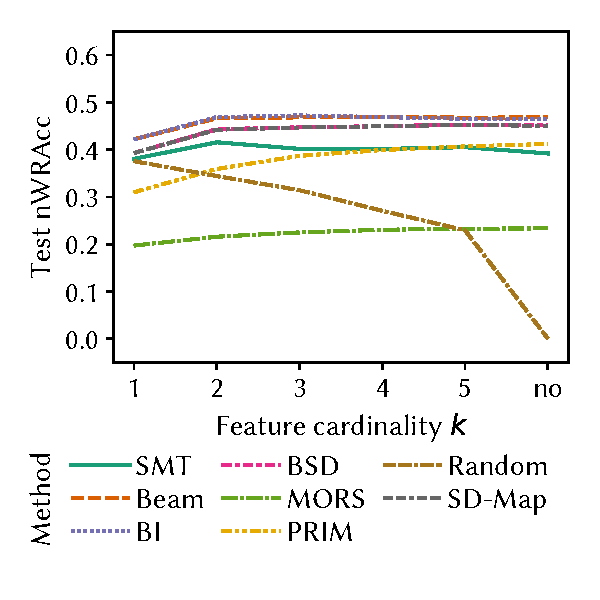
\includegraphics[width=\textwidth, trim=10 25 10 10, clip]{plots/csd-cardinality-test-nwracc-all-datasets.pdf}
			\caption{All 27 datasets, test set.}
			\label{fig:csd:cardinality-test-nwracc-all-datasets}
			%JB: "BSD" and "SD-Map" get closer to "Beam" and "BI" (particulalrly for higher "k"), better than "SMT"
			%JB: reason: less overfitting (probably due to reduced search space), while "SMT" shows highest overfitting (train-test diff in quality)
			%JB: quality increase over "k" also smaller due to overfitting
		\end{subfigure}
		\caption*{
			Mean subgroup quality over datasets and cross-validation folds, by subgroup-discovery method and feature cardinality~$k$.
			Results from the search for original subgroups.
		}
		\label{fig:csd:cardinality}
	\end{figure}
\end{frame}

\begin{frame}[t]{Results -- Alternative Subgroup Descriptions}
	\begin{figure}[t]
		\centering
		\begin{subfigure}[t]{0.32\textwidth}
			\centering
			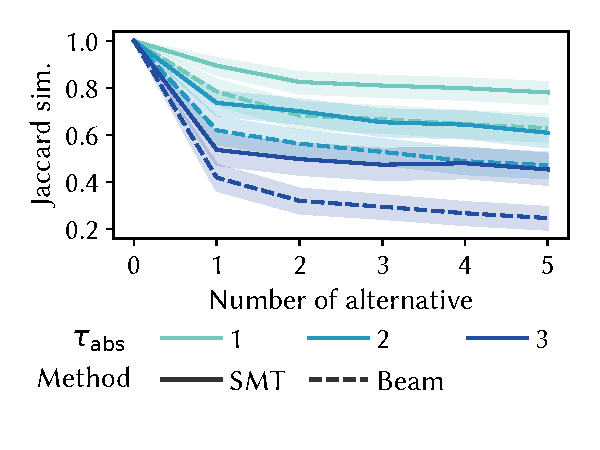
\includegraphics[width=\textwidth, trim=10 25 10 10, clip]{plots/csd-alternatives-jaccard.pdf}
			\caption{Jaccard similarity.}
			\label{fig:csd:alternatives-jaccard}
			%JB: here two just subgroup-discovery methods (our solver-based, one heuristic)
			%JB: alternative subgroup descriptions less (data-object) similar to original the more alternatives desired and the higher (feature-selection) dissimilarity threshold
			%JB: strongest decrease to first alternative
		\end{subfigure}
		\hfill
		\begin{subfigure}[t]{0.32\textwidth}
			\centering
			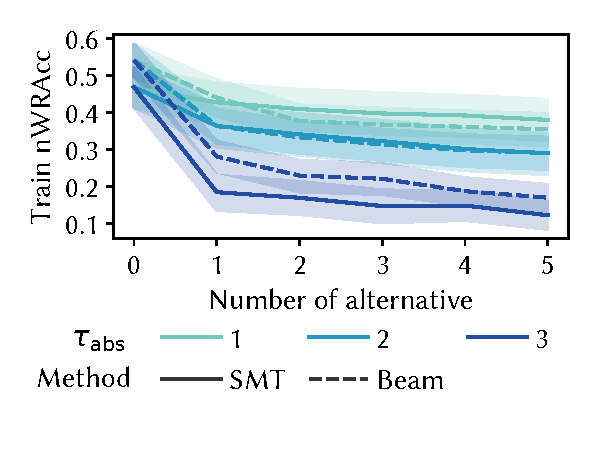
\includegraphics[width=\textwidth, trim=10 25 10 10, clip]{plots/csd-alternatives-train-nwracc.pdf}
			\caption{Training-set subgroup quality (nWRAcc).}
			\label{fig:csd:alternatives-train-nwracc}
			%JB: similar trends for subgroup quality
			%JB: heuristics similar or better quality than solver-based approach (while for Jaccard similarity, SMT seemed better, but that does not even transfer to Hamming similarity)
		\end{subfigure}
		\hfill
		\begin{subfigure}[t]{0.32\textwidth}
			\centering
			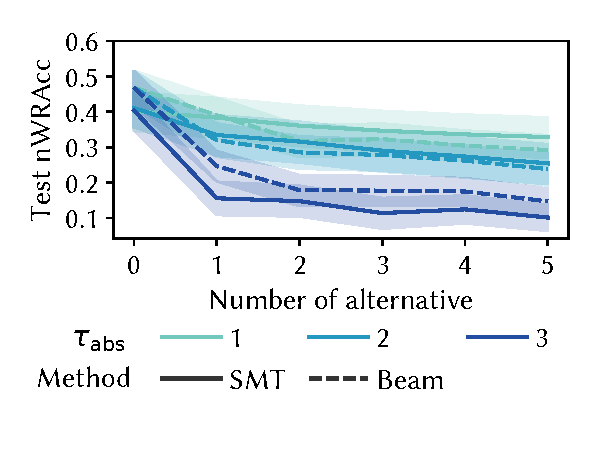
\includegraphics[width=\textwidth, trim=10 25 10 10, clip]{plots/csd-alternatives-test-nwracc.pdf}
			\caption{Test-set subgroup quality (nWRAcc).}
			\label{fig:csd:alternatives-test-nwracc}
		\end{subfigure}
		\caption*{
			Mean similarity and quality of alternative subgroup descriptions, with 95\% confidence intervals based on datasets and cross-validation folds, by subgroup-discovery method, number of alternative, and dissimilarity threshold~$\tau_{\text{abs}}$.
		}
		\label{fig:csd:alternatives}
	\end{figure}
\end{frame}

\begin{frame}[t]{Summary}
	\begin{itemize}
		\item \textbf{Goal:} Introduce and analyze two constraint types to foster interpretability of subgroup descriptions
		\begin{itemize}
			\item Limit number of features used in subgroup description
			\item Find alternative subgroup descriptions
		\end{itemize}
		\pause
		\vspace{\baselineskip}
		\item \textbf{Contributions:} Formalization (as SMT problem), complexity analyses, and experiments
		\pause
		\vspace{\baselineskip}
		\item \textbf{Experimental results:}
		\begin{itemize}
			\item Heuristic search methods yield close-to-optimal subgroup quality in short time
			\item Subgroup descriptions using few features yield similar subgroup quality as those using many features
			\item Different subgroup descriptions (used features) may capture similar subgroup (set of data objects)
		\end{itemize}
		\pause
		\vspace{\baselineskip}
		\item \textbf{Resources:}
		\begin{itemize}
			\item Paper~\cite{bach2025subgroup} (longer arXiv version~\cite{bach2025using})
			%JB: all main results are included in conference version
			\item Code~\cite{bach2025constrained} (including Python package \texttt{csd} with six subgroup-discovery methods)
			%JB: we implemented six methods from scratch, while two (BSD and SD-Map) were wrapped from another package (SD4Py)
			\item Experimental data~\cite{bach2025experimental}
		\end{itemize}
	\end{itemize}
\end{frame}

\appendix
\beginbackup % subsequent slides do not impact overall slide count

\begin{frame}[plain]
	\centering
	\Huge Appendix
\end{frame}

\begin{frame}[t]{Formalization -- Alternative Subgroup Descriptions}
	\begin{itemize}
		\item \textbf{Concept:} Cover similar set of data objects as given subgroup with different set of selected features
		\begin{itemize}
			\item Repeat sequentially to get $a \in \mathbb{N}$ alternatives for dissimilarity threshold~$\tau \in \mathbb{R}_{\geq 0}$
		\end{itemize}
		\vspace{\baselineskip}
		\item \textbf{Chosen optimization objective:} Maximize normalized Hamming similarity (= prediction accuracy)
		%JB: new objective! don't optimize subgroup quality anymore
		\begin{equation*}
			\text{sim}_{\text{nHamm}}(b^{(a)}, b^{(0)}) = \frac{1}{m} \cdot \sum_{i=1}^m \left( b_i^{(a)} \leftrightarrow b_i^{(0)} \right) = \frac{1}{m} \cdot \Big( \sum\limits_{\substack{i \in \{1, \dots, m\} \\ b_i^{(0)} = 1}} b_i^{(a)} + \sum\limits_{\substack{i \in \{1, \dots, m\} \\ b_i^{(0)} = 0}} \lnot b_i^{(a)} \Big)
			%JB: reminder: b_i denotes whether data object in subgroup or not
			%JB: (0) is orignal subgroup, (a) the alternative
			%JB: is linear (logical NOT can be linearized easily), while Jaccard similarity is not
		\end{equation*}
		\vspace{\baselineskip}
		\item \textbf{Chosen dissimilarity constraints:} From each existing feature set, deselect at least $\tau_{\text{abs}} \in \mathbb{N}$ (but $\leq k$) features
		%JB: "deselect": do not select again
		\begin{equation*}
			\forall l \in \{0, \dots, a-1\}:~ \text{dis}_{\text{des}}(s^{(a)}, s^{(l)}) = \sum_{\substack{j \in \{1, \dots, n\} \\ s^{(l)}_j = 1}} \lnot s^{(a)}_j \geq \min \left( \tau_{\text{abs}},~k^{(l)} \right)
			%JB: min prevents infeasibility
			%JB: not a commonly used measure, not even symmetric
			%JB: however, linear and antimonotonic (Dice and Jaccard are not), which eases integration into solver and heuristics
		\end{equation*}
		%JB: other constraints from subgroup discovery remain in problem as is
	\end{itemize}
\end{frame}

\begin{frame}[t]{Computational Complexity}
	\begin{itemize}
		\item Subgroup discovery with a feature-cardinality constraint is $\mathcal{NP}$-complete
		\vspace{\baselineskip}
		\item \textbf{Proof:} Reduction from \textsc{Set Covering}~\cite{karp1972reducibility}
		\begin{itemize}
			\item Set-covering problem: Given set of elements~$E = \{e_1, \dots, e_m\}$, set of sets~$\mathbb{S} = \{S_1,  \dots, S_n\}$ with $E = \bigcup_{S \in \mathbb{S}} S$, and a cardinality~$k \in \mathbb{N}$, does subset $\mathbb{C} \subseteq \mathbb{S}$ with $|\mathbb{C}| \leq k$ and $E = \bigcup_{S \in \mathbb{C}} S$ exist?
			\item Perfect-subgroup discovery: Find subgroup containing all positive data objects ($y_i = 1$) and zero negatives ($y_i = 0$)
			%JB: may not exist, i.e., search problem instead of optimization problem
			\item Problem transformation:
			%JB: from set covering to perfect-subgroup discovery
			\begin{itemize}
				\item Dataset~$X \in \{0, 1\}^{(m + 1) \times n}$ with $X_{ij} := (e_i \in S_j)$
				%JB: elements become data objects, sets become features, set membership becomes feature value
				%JB: binary is special case of real-valued
				\item Data Object $m+1$ represents an element not contained in any set, i.e., $X_{(m+1)j} = 0$ for all~$j \in \{1, \dots, n\}$
				\item Prediction target $y \in \{0, 1\}^{m+1}$ with $y_{m+1} = 1$ and $y_i = 0$ otherwise
				%JB: indicates whether not contained in any set
				%JB: further, parameter "k" remains as-is
			\end{itemize}
			\item Perfect subgroup only contains Data Object $m+1$ and uses $\mathit{lb}_j = \mathit{ub}_j = 0$ conditions for selected features
			%JB: new data object only has 0 as feature values
			%JB: bounds [0, 1] represent unselected features
			\item Other data objects have value 1 for at least one selected feature $\rightarrow$ each element is in a selected set
			\item I.e., algorithm for perfect-subgroup discovery also solves \textsc{Set Covering}
			%JB: however, latter is NP-hard, so former is NP-hard as well (and NP-complete since in NP)
			\item Finally, optimizing subgroup quality typically at least as hard as finding perfect subgroup
			%JB: depends on notion of subgroup quality, but mild condition (perfect subgroup is unique optimum if exists), satisfied for WRAcc
		\end{itemize}
		\vspace{\baselineskip}
		\item Finding alternative subgroup descriptions with a feature-cardinality constraint is $\mathcal{NP}$-complete as well
	\end{itemize}
\end{frame}

\begin{frame}[t]{Results -- Solver Timeouts}
	\begin{figure}
		\centering
		\begin{subfigure}[t]{0.32\textwidth}
			\centering
			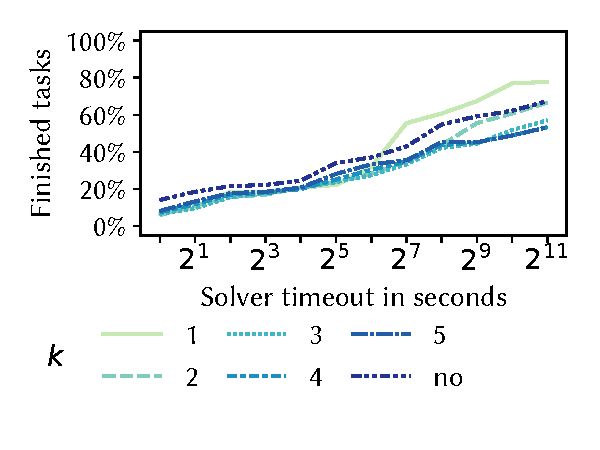
\includegraphics[width=\textwidth, trim=10 25 10 10, clip]{plots/csd-timeouts-finished-tasks.pdf}
			\caption{
				Frequency of finished \emph{SMT} tasks over datasets and cross-validation folds, by feature cardinality~$k$.
			}
			\label{fig:csd:timeouts-finished-tasks}
			%JB: increase of finished tasks with timeout, and decreasing marginal gain (note logarithmic x-axis) -> may tasks finish fast, but some take really long
		\end{subfigure}
		\hspace{1cm}
		\begin{subfigure}[t]{0.32\textwidth}
			\centering
			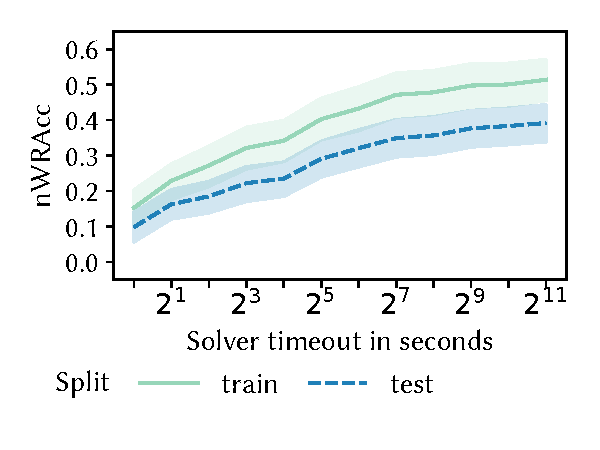
\includegraphics[width=\textwidth, trim=10 25 10 10, clip]{plots/csd-timeouts-nwracc.pdf}
			\caption{
				Mean subgroup quality, with 95\% confidence intervals based on datasets and cross-validation folds.
				Results without a feature-cardinality constraint.
			}
			\label{fig:csd:timeouts-nwracc}
			%JB: subgroup quality also shows decreasing marginal gain
		\end{subfigure}
		\caption*{
			Impact of solver timeouts for \emph{SMT} as the subgroup-discovery method.
			Results from the search for original subgroups.
		}
		\label{fig:csd:timeouts}
	\end{figure}
\end{frame}

\begin{frame}[t]{Results -- Runtime}
	\begin{columns}[T]
		\begin{column}{\kitthreecolumns}
			\begin{table}
				\centering
				\caption*{
					Mean runtime (in seconds) over datasets and cross-validation folds, by subgroup-discovery method and feature cardinality~$k$.
					Results from the search for original subgroups.
				}
				\begin{tabular}{lrrrrrr}
					\toprule
					$k$ & 1 & 2 & 3 & 4 & 5 & no \\
					\midrule
					BI & 7.8 & 11.7 & 14.2 & 16.7 & 18.7 & 35.0 \\
					BSD & 0.9 & 0.9 & 0.9 & 2.7 & 29.5 & 55.7 \\
					Beam & 6.8 & 10.1 & 12.8 & 14.6 & 16.1 & 30.5 \\
					MORS & 0.0 & 0.0 & 0.0 & 0.0 & 0.0 & 0.0 \\
					PRIM & 0.1 & 0.2 & 0.3 & 0.3 & 0.5 & 1.3 \\
					Random & 0.6 & 0.6 & 0.6 & 0.7 & 0.7 & 0.9 \\
					SD-Map & 2.3 & 3.3 & 9.6 & 54.0 & 345.2 & 367.4 \\
					SMT & 648.2 & 911.3 & 1091.7 & 1113.4 & 1117.4 & 849.0 \\
					\bottomrule
				\end{tabular}
				\label{tab:csd:cardinality-runtime}
				%JB: "SMT" one to two orders of magnitude slower than "Beam"/"BI" (which yield better quality) and "BSD"/"SD-Map"
				%JB: "Beam"/"BI" are one to two oders of magnitude slower than "PRIM"/"Random"
				%JB: new baseline "MORS" practically finishes at once -> good for an initial lower bound on quality
				%JB: among heuristics, "PRIM" fastest but also worst quality (tradeoff)
				%JB: heuristics and "BSD"/SD-Map" speed up with smaller "k", "SMT" less clear (increase till k=3, stable for K=4 and k=5, unconstrained faster again)
			\end{table}
		\end{column}
		\begin{column}{\kitthreecolumns}
			\begin{table}[t]
				\centering
				\caption*{
					Mean runtime (in seconds) over datasets and cross-validation folds, by subgroup-discovery method, dissimilarity threshold~$\tau_{\text{abs}}$, and number of alternative.
					Results from the search for alternative subgroup descriptions.
				}
				\begin{tabular}{llrrrrrr}
					\toprule
					\multirow{2}{*}{Method} & \multirow{2}{*}{$\tau_{\text{abs}}$} & \multicolumn{6}{c}{Number of alternative} \\
					\cmidrule(lr){3-8}
					& & 0 & 1 & 2 & 3 & 4 & 5 \\
					\midrule
					\multirow[t]{3}{*}{Beam} & 1 & 12.8 & 8.0 & 7.6 & 7.3 & 7.3 & 7.3 \\
					& 2 & 12.8 & 7.7 & 7.4 & 7.2 & 7.0 & 6.8 \\
					& 3 & 12.8 & 5.8 & 5.1 & 4.7 & 4.1 & 3.5 \\
					\multirow[t]{3}{*}{SMT} & 1 & 1091.7 & 166.0 & 221.5 & 239.6 & 258.1 & 277.9 \\
					& 2 & 1105.2 & 377.5 & 463.5 & 537.5 & 599.4 & 658.3 \\
					& 3 & 1107.4 & 869.1 & 670.8 & 597.6 & 588.1 & 557.6 \\
					\bottomrule
				\end{tabular}
				\label{tab:csd:alteratives-runtime}
				%JB: search for alternatives faster than for original subgroup
				%JB: "Beam" again one to orders of magnitude faster than "SMT"
				%JB: "Beam" decreasing runtime over number of alternatives and dissimilarity
				%JB: "SMT" has increasing runtime over number of alternatives if overlap allowed and decreasing if forbidden
			\end{table}
		\end{column}
	\end{columns}
\end{frame}

\begin{frame}[t, allowframebreaks]{References}
	\printbibliography
\end{frame}

\backupend

\end{document}
